\documentclass[
  aspectratio=169,
]{beamer}

\usepackage[english]{babel}
\usepackage[utf8]{inputenc}
\usepackage[T1]{fontenc}
\usepackage{booktabs}
\usepackage{array}
\usepackage{listings}
\usepackage{csquotes}
\usepackage[backend=bibtex,style=numeric]{biblatex}
\usetheme[
  workplace=fi,
]{MU}

\graphicspath{{../text/assets/}{generated/}}
\addbibresource{slides.bib}

\title[Generative Neural Models for SVG]{Generative Neural Models\\for Scalable Vector Graphics}
\author[J.\,Kuchař]{Josef Kuchař\texorpdfstring{\\}{, }567769@mail.muni.cz}
\institute[FI MU]{Faculty of Informatics, Masaryk University\texorpdfstring{\\[.5em]\scriptsize Advisor: Mgr. Michal Štefánik, Ph.D.\\Consultant: Mgr. Marek Kadlčík}{}}
\date{June 18, 2026}
\subject{Master's Thesis Defense}
\keywords{scalable vector graphics, text-to-vector generation, neural vectorization}

\newcommand{\tightitems}{\setlength{\itemsep}{0.35em}}
\newcommand{\smallimg}[1]{\includegraphics[width=.085\textwidth,height=.085\textwidth,keepaspectratio]{#1}}
\newcommand{\stageoneimg}[1]{\raisebox{-.5\height}{\smallimg{#1}}}
\newcommand{\tinyimg}[1]{\includegraphics[width=.066\textwidth,height=.066\textwidth,keepaspectratio]{#1}}
\newcommand{\dataimg}[1]{\includegraphics[width=.15\textwidth,height=.15\textwidth,keepaspectratio]{#1}}
\newcommand{\svgout}[1]{\fbox{\includegraphics[width=.068\textwidth,height=.068\textwidth,keepaspectratio]{#1}}}
\newcommand{\plainout}[1]{\includegraphics[width=.068\textwidth,height=.068\textwidth,keepaspectratio]{#1}}
\newcommand{\thanksimg}[1]{\includegraphics[width=.5\textwidth,height=.5\textwidth,keepaspectratio]{#1}}
\newcommand{\metricbest}[1]{\textbf{#1}}

\lstdefinestyle{svgcode}{
  basicstyle=\ttfamily\tiny,
  columns=fullflexible,
  keywordstyle=\color{blue!70!black},
  stringstyle=\color{orange!80!black},
  identifierstyle=\color{green!45!black},
  alsoletter={-},
  morekeywords={svg,rect,circle,path,viewBox,x,y,width,height,fill,cx,cy,r,d,stroke,stroke-width,stroke-linecap},
  morestring=[b]",
  showstringspaces=false
}

\begin{document}

\begin{frame}[plain]
\maketitle
\end{frame}

\section{Motivation}

\begin{frame}[fragile]{SVG}
\begin{columns}[T,onlytextwidth]
  \begin{column}{.52\textwidth}
    \begin{itemize}
      \tightitems
      \item Native format for icons, logos, illustrations, diagrams, and UI assets
      \item Resolution independence, compactness, and editability
    \end{itemize}
  \end{column}
  \begin{column}{.42\textwidth}
    \centering
    
\includegraphics[width=.95\linewidth,height=.4\textheight,keepaspectratio]{svg_primitives_example.pdf}

    \vspace{.6em}
    \begin{lstlisting}[style=svgcode]
<svg viewBox="0 0 120 80">
  <rect x="12" y="14" width="32" height="32"
        fill="#f97316"/>
  <circle cx="80" cy="30" r="18"
          fill="#22c55e"/>
  <path d="M 18 66 C 42 44, 76 86, 104 58"
        fill="none" stroke="#2563eb"
        stroke-width="6" stroke-linecap="round"/>
</svg>
    \end{lstlisting}
  \end{column}
\end{columns}
\end{frame}

\begin{frame}{Objective}
\begin{itemize}
  \tightitems
  \item Design, implement, and evaluate a modular text-to-SVG pipeline
\end{itemize}

\vspace{1.0em}
\centering
\begin{tabular}{c@{\hspace{1.4em}$\longrightarrow$\hspace{1.4em}}c}
  \begin{minipage}{.28\textwidth}
    \centering
    \large \texttt{"a simple lighthouse icon"}

    \vspace{.35em}
    \scriptsize \textcolor{blue}{Prompt}
  \end{minipage}
  &
  \begin{minipage}{.28\textwidth}
    \centering
    \fbox{
\includegraphics[width=.85\linewidth,height=.34\textheight,keepaspectratio]{lighthouse.pdf}}

    \vspace{.35em}
    \scriptsize \textcolor{blue}{SVG}
  \end{minipage}
\end{tabular}
\end{frame}

\begin{frame}{Central Problem}
\begin{itemize}
  \tightitems
  \item semantic grounding from text
  \item visual composition
  \item geometric structure
  \item valid SVG syntax and rendering behavior
\end{itemize}
\end{frame}

\begin{frame}{Previous text-to-SVG work}
\centering
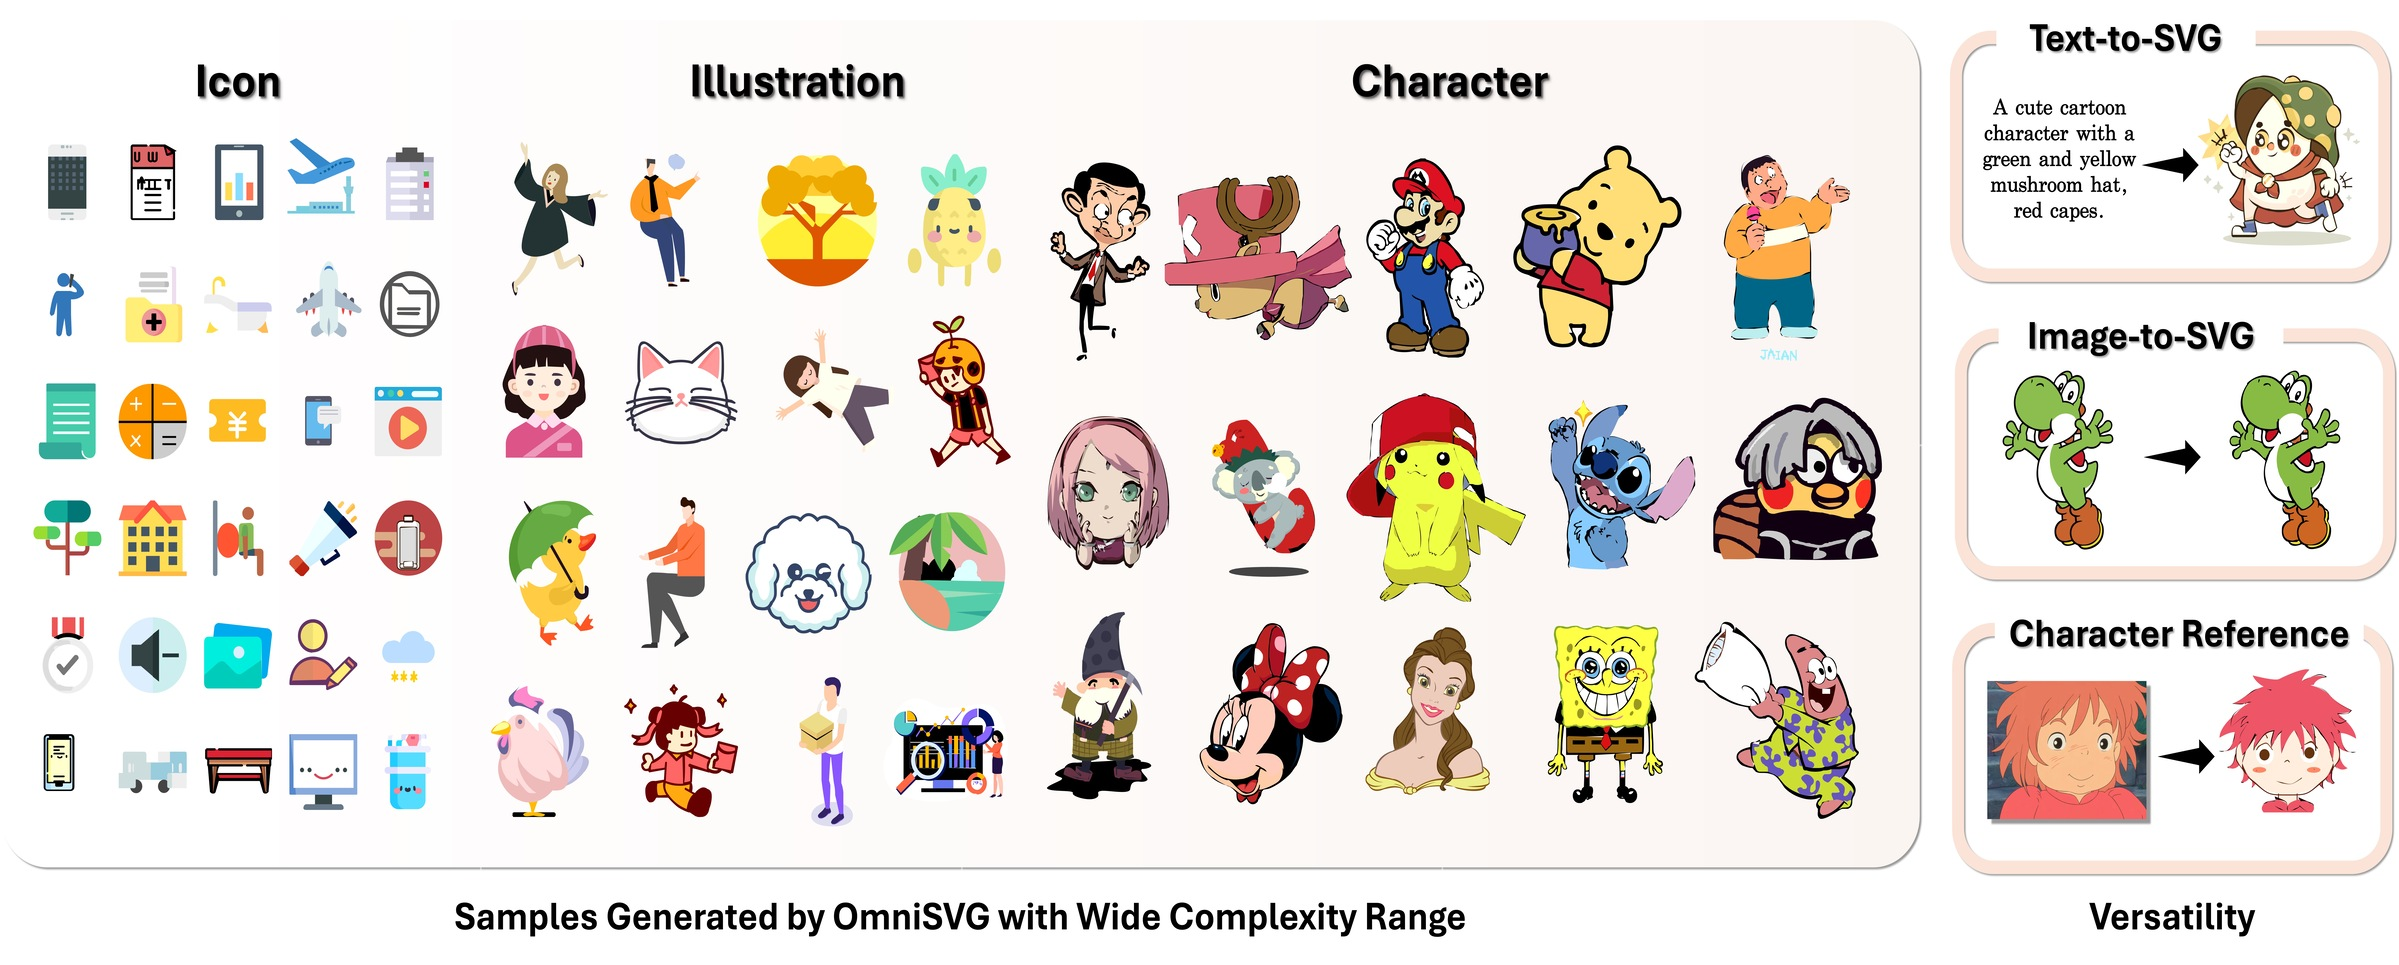
\includegraphics[width=.95\textwidth,height=.43\textheight,keepaspectratio]{omnisvg_teaser.jpg}

\vspace{.2em}
{\tiny Source: OmniSVG~\cite{yang2025omnisvg}}

\vspace{.45em}
\begin{tabular}{c@{\hspace{1.4em}$\longrightarrow$\hspace{1.4em}}c}
  \begin{minipage}{.23\textwidth}
    \centering
    \footnotesize \texttt{"A minimal rocket icon"}

    \vspace{.25em}
    \tiny \textcolor{blue}{Prompt}
  \end{minipage}
  &
  \begin{minipage}{.18\textwidth}
    \centering
    \fbox{\includegraphics[width=.8\linewidth,height=.15\textheight,keepaspectratio]{omnisvg4_rocket.pdf}}

    \vspace{.25em}
    \tiny \textcolor{blue}{SVG}
  \end{minipage}
\end{tabular}
\end{frame}

\begin{frame}{Diffusion models}
\centering
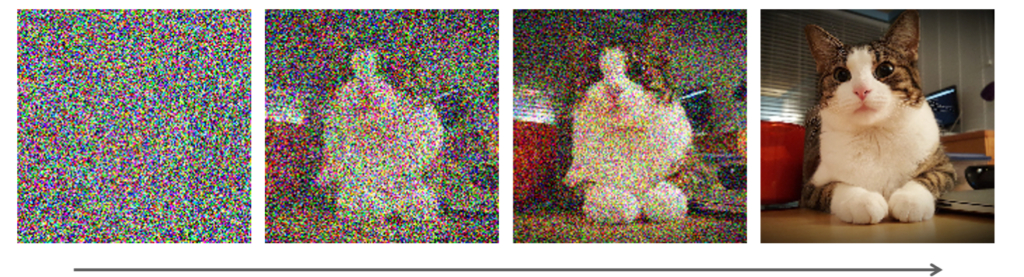
\includegraphics[width=.95\textwidth,height=.43\textheight,keepaspectratio]{assets/diffusion.jpg}

\vspace{.85em}
\begin{tabular}{c@{\hspace{1.4em}$\longrightarrow$\hspace{1.4em}}c}
  \begin{minipage}{.23\textwidth}
    \centering
    \footnotesize \texttt{"A minimal rocket icon"}

    \vspace{.25em}
    \tiny \textcolor{blue}{Prompt}
  \end{minipage}
  &
  \begin{minipage}{.18\textwidth}
    \centering
    \fbox{
\includegraphics[width=.8\linewidth,height=.15\textheight,keepaspectratio]{assets/z-image-rocket-icon.jpeg}}

    \vspace{.25em}
    \tiny \textcolor{blue}{Raster image}
  \end{minipage}
\end{tabular}
\end{frame}

\section{Pipeline}

\begin{frame}{Two-Stage Pipeline}
\centering

\includegraphics[width=.95\textwidth,height=.72\textheight,keepaspectratio]{assets/pipeline.pdf}
\end{frame}

\begin{frame}{Stage 1: Raster Generation}
\begin{columns}[T,onlytextwidth]
  \begin{column}{.47\textwidth}
    \begin{itemize}
      \tightitems
      \item Pretrained Z-Image text-to-image model
      \item SVG-style prompt prefix and LoRA fine-tuning
    \end{itemize}
  \end{column}
  \begin{column}{.48\textwidth}
    \centering
    \scriptsize
    \begin{tabular}{lccc}
      \toprule
      Variant & CLIP $\uparrow$ & DINO $\uparrow$ & MSE $\downarrow$ \\
      \midrule
      Base & .818 & .509 & 266.6 \\
      Base + prefix & .820 & .546 & 230.2 \\
      Base + prefix + LoRA & \metricbest{.883} & \metricbest{.617} & 145.5 \\
      Turbo + prefix & .871 & .584 & \metricbest{142.7} \\
      Turbo + prefix + LoRA & .879 & .600 & 143.2 \\
      \bottomrule
    \end{tabular}
  \end{column}
\end{columns}

\end{frame}

\begin{frame}{Stage 1: Qualitative Results}
\centering
\begin{tabular}{lcccc}
\scriptsize Reference &
   \stageoneimg{raster/reference/0001.png} & \stageoneimg{raster/reference/0002.png} &
   \stageoneimg{raster/reference/0003.png} & \stageoneimg{raster/reference/0004.png} \\
\noalign{\vskip 1.2em}
\scriptsize Z-Image Base &
   \stageoneimg{raster/base/0001.png} & \stageoneimg{raster/base/0002.png} &
   \stageoneimg{raster/base/0003.png} & \stageoneimg{raster/base/0004.png} \\
\noalign{\vskip 1.2em}
\scriptsize Base + prefix + LoRA &
   \stageoneimg{raster/base_prefixed_lora/0001.png} & \stageoneimg{raster/base_prefixed_lora/0002.png} &
   \stageoneimg{raster/base_prefixed_lora/0003.png} & \stageoneimg{raster/base_prefixed_lora/0004.png} \\
\end{tabular}
\end{frame}

\section{Vectorization}

\begin{frame}{Stage 2: Bezier Representation}
\begin{columns}[T,onlytextwidth]
  \begin{column}{.5\textwidth}
    \begin{itemize}
      \tightitems
      \item Fixed-size cubic Bezier representation
      \item Flow-compatible dimensionality
      \item Direct rendering to SVG paths
      \item Constrained capacity and primitive semantics
    \end{itemize}
  \end{column}
  \begin{column}{.44\textwidth}
    \centering
    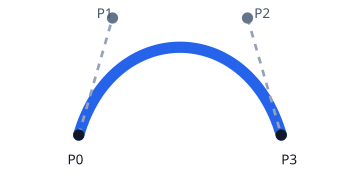
\includegraphics[width=.92\linewidth,height=.6\textheight,keepaspectratio]{svg_bezier_example.pdf}
  \end{column}
\end{columns}
\end{frame}

\begin{frame}{Stage 2: Conditional Flow-Matching Vectorizer}
\centering

\includegraphics[width=.95\textwidth,height=.7\textheight,keepaspectratio]{assets/architecture.pdf}
\end{frame}

\begin{frame}{Training Data}
\begin{columns}[T,onlytextwidth]
  \begin{column}{.48\textwidth}
    \centering
    \structure{SVG-derived data}

    \vspace{.7em}
    \setlength{\tabcolsep}{0pt}
    \begin{tabular}{ccc}
      \dataimg{svg_repo_dataset/svg_repo_01.png} &
      \dataimg{svg_repo_dataset/svg_repo_02.png} &
      \dataimg{svg_repo_dataset/svg_repo_03.png} \\
      \dataimg{svg_repo_dataset/svg_repo_04.png} &
      \dataimg{svg_repo_dataset/svg_repo_05.png} &
      \dataimg{svg_repo_dataset/svg_repo_06.png} \\
      \dataimg{svg_repo_dataset/svg_repo_07.png} &
      \dataimg{svg_repo_dataset/svg_repo_08.png} &
      \dataimg{svg_repo_dataset/svg_repo_09.png}
    \end{tabular}
  \end{column}
  \begin{column}{.48\textwidth}
    \centering
    \structure{Synthetic Bezier data}

    \vspace{.7em}
    \setlength{\tabcolsep}{0pt}
    \begin{tabular}{ccc}
      \dataimg{syntetic_generator/synthetic_generator_01.png} &
      \dataimg{syntetic_generator/synthetic_generator_02.png} &
      \dataimg{syntetic_generator/synthetic_generator_03.png} \\
      \dataimg{syntetic_generator/synthetic_generator_04.png} &
      \dataimg{syntetic_generator/synthetic_generator_05.png} &
      \dataimg{syntetic_generator/synthetic_generator_06.png} \\
      \dataimg{syntetic_generator/synthetic_generator_07.png} &
      \dataimg{syntetic_generator/synthetic_generator_08.png} &
      \dataimg{syntetic_generator/synthetic_generator_09.png}
    \end{tabular}
  \end{column}
\end{columns}
\end{frame}

\begin{frame}{Architecture Ablation}
\begin{columns}[T,onlytextwidth]
  \begin{column}{.55\textwidth}
    \centering
    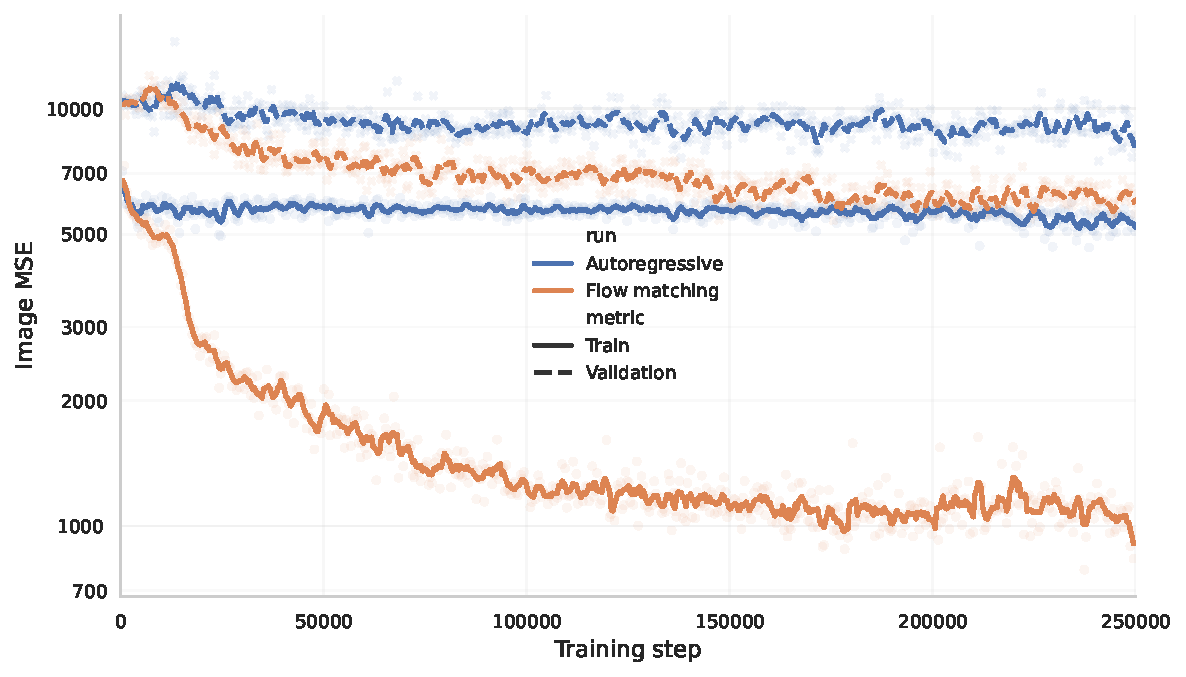
\includegraphics[width=\linewidth,height=.63\textheight,keepaspectratio]{wandb/flow-matching-vs-autoregressive_image_mse.pdf}
  \end{column}
  \begin{column}{.39\textwidth}
    \begin{itemize}
      \tightitems
      \item Same model scale and image encoder
      \item Stepwise Bezier prediction for autoregressive baseline
      \item Lower image-space error with flow matching
    \end{itemize}
  \end{column}
\end{columns}
\end{frame}

\begin{frame}{Vectorization Benchmark}
\centering
\begin{tabular}{lcccccc}
 & \tinyimg{vectorization_qualitative/synthetic/reference/0000.png}
 & \tinyimg{vectorization_qualitative/synthetic/reference/0001.png}
 & \tinyimg{vectorization_qualitative/synthetic/reference/0002.png}
 & \tinyimg{vectorization_qualitative/synthetic/reference/0003.png}
 & \tinyimg{vectorization_qualitative/synthetic/reference/0004.png}
 & \tinyimg{vectorization_qualitative/synthetic/reference/0005.png} \\
\scriptsize Reference \\
 & \tinyimg{vectorization_qualitative/synthetic/proposed/0000.png}
 & \tinyimg{vectorization_qualitative/synthetic/proposed/0001.png}
 & \tinyimg{vectorization_qualitative/synthetic/proposed/0002.png}
 & \tinyimg{vectorization_qualitative/synthetic/proposed/0003.png}
 & \tinyimg{vectorization_qualitative/synthetic/proposed/0004.png}
 & \tinyimg{vectorization_qualitative/synthetic/proposed/0005.png} \\
\scriptsize Ours 0.26B \\
 & \tinyimg{vectorization_qualitative/synthetic/starvector_1b/0000.png}
 & \tinyimg{vectorization_qualitative/synthetic/starvector_1b/0001.png}
 & \tinyimg{vectorization_qualitative/synthetic/starvector_1b/0002.png}
 & \tinyimg{vectorization_qualitative/synthetic/starvector_1b/0003.png}
 & \tinyimg{vectorization_qualitative/synthetic/starvector_1b/0004.png}
 & \tinyimg{vectorization_qualitative/synthetic/starvector_1b/0005.png} \\
\scriptsize StarVector 1B \\
 & \tinyimg{vectorization_qualitative/synthetic/omnisvg_4b/0000.png}
 & \tinyimg{vectorization_qualitative/synthetic/omnisvg_4b/0001.png}
 & \tinyimg{vectorization_qualitative/synthetic/omnisvg_4b/0002.png}
 & \tinyimg{vectorization_qualitative/synthetic/omnisvg_4b/0003.png}
 & \tinyimg{vectorization_qualitative/synthetic/omnisvg_4b/0004.png}
 & \tinyimg{vectorization_qualitative/synthetic/omnisvg_4b/0005.png} \\
\scriptsize OmniSVG 4B \\
\end{tabular}
\end{frame}

\begin{frame}{Vectorization Metrics}
\small
\begin{columns}[T,onlytextwidth]
  \begin{column}{.52\textwidth}
    \structure{Synthetic rendered fidelity}

    \vspace{.3em}
    \begin{tabular}{lccc}
      \toprule
      Method & MSE $\downarrow$ & SSIM $\uparrow$ & IoU $\uparrow$ \\
      \midrule
      Ours 0.26B & \metricbest{2432.6} & \metricbest{.725} & \metricbest{.758} \\
      OmniSVG 4B & 9591.5 & .330 & .432 \\
      StarVector 1B & 6339.1 & .314 & .297 \\
      \midrule
      vtracer & 24.0 & .997 & .993 \\
      \bottomrule
    \end{tabular}
  \end{column}
  \begin{column}{.43\textwidth}
    \structure{Validity and compactness}

    \vspace{.3em}
    \begin{tabular}{lcc}
      \toprule
      Method & Valid & Commands \\
      \midrule
      Ours 0.26B & \metricbest{100\%} & \metricbest{90} \\
      OmniSVG 4B & 99\% & 394 \\
      StarVector 1B & 43\% & 447 \\
      \midrule
      vtracer & 100\% & 625 \\
      \bottomrule
    \end{tabular}
  \end{column}
\end{columns}

\vspace{.8em}
\begin{block}{Main trade-off}
Classical tracing gives the best pixel fidelity; the proposed neural vectorizer trades fidelity for compact, valid structured output.
\end{block}
\end{frame}

\section{End-to-End Evaluation}

\begin{frame}{Generated Raster Vectorization}
\centering
\begin{tabular}{lcccccc}
 & \tinyimg{z_image_vectorization/reference/0000.png}
 & \tinyimg{z_image_vectorization/reference/0001.png}
 & \tinyimg{z_image_vectorization/reference/0002.png}
 & \tinyimg{z_image_vectorization/reference/0003.png}
 & \tinyimg{z_image_vectorization/reference/0004.png}
 & \tinyimg{z_image_vectorization/reference/0005.png} \\
\scriptsize Raster input \\
 & \tinyimg{z_image_vectorization/proposed/0000.png}
 & \tinyimg{z_image_vectorization/proposed/0001.png}
 & \tinyimg{z_image_vectorization/proposed/0002.png}
 & \tinyimg{z_image_vectorization/proposed/0003.png}
 & \tinyimg{z_image_vectorization/proposed/0004.png}
 & \tinyimg{z_image_vectorization/proposed/0005.png} \\
\scriptsize Ours 0.26B \\
 & \tinyimg{z_image_vectorization/starvector_1b/0000.png}
 & \tinyimg{z_image_vectorization/starvector_1b/0001.png}
 & \tinyimg{z_image_vectorization/starvector_1b/0002.png}
 & \tinyimg{z_image_vectorization/starvector_1b/0003.png}
 & \tinyimg{z_image_vectorization/starvector_1b/0004.png}
 & \tinyimg{z_image_vectorization/starvector_1b/0005.png} \\
\scriptsize StarVector 1B \\
 & \tinyimg{z_image_vectorization/vtracer/0000.png}
 & \tinyimg{z_image_vectorization/vtracer/0001.png}
 & \tinyimg{z_image_vectorization/vtracer/0002.png}
 & \tinyimg{z_image_vectorization/vtracer/0003.png}
 & \tinyimg{z_image_vectorization/vtracer/0004.png}
 & \tinyimg{z_image_vectorization/vtracer/0005.png} \\
\scriptsize vtracer \\
\end{tabular}
\end{frame}

\begin{frame}{End-to-End Text-to-SVG Examples}
\centering
{
\setlength{\tabcolsep}{.75em}
\renewcommand{\arraystretch}{1.25}
\begin{tabular}{
  >{\centering\arraybackslash\scriptsize}m{.28\textwidth}
  >{\centering\arraybackslash}m{.13\textwidth}
  >{\centering\arraybackslash}m{.13\textwidth}
  >{\centering\arraybackslash}m{.13\textwidth}
}
\scriptsize\textbf{Prompt} & \scriptsize\textbf{Proposed pipeline} & \scriptsize\textbf{OmniSVG 4B} & \scriptsize\textbf{OmniSVG 8B} \\[.45em]
\scriptsize a simple lighthouse icon & \plainout{lighthouse.pdf} & \plainout{omnisvg4_lighthouse.pdf} & \plainout{omnisvg8_lighthouse.pdf} \\
\scriptsize A minimal rocket icon & \plainout{rocket.pdf} & \plainout{omnisvg4_rocket.pdf} & \plainout{omnisvg8_rocket.pdf} \\
\scriptsize A cute cat face icon & \plainout{cat.pdf} & \plainout{omnisvg4_cat.pdf} & \plainout{omnisvg8_cat.pdf} \\
\scriptsize A magic potion bottle with bubbles, sparkles, cork, and label & \plainout{potion.pdf} & \plainout{omnisvg4_potion.pdf} & \plainout{omnisvg8_potion.pdf} \\
\end{tabular}
}
\end{frame}

\section{Conclusion}

\begin{frame}{Contributions}
\begin{itemize}
  \tightitems
  \item Two-stage text-to-SVG pipeline
  \item Conditional flow-matching Bezier vectorizer
  \item Synthetic Bezier data generator
  \item Fidelity, validity, compactness, and editability evaluation
\end{itemize}
\end{frame}

\begin{frame}{Limitations}
\begin{itemize}
  \tightitems
  \item Bezier-only geometry without primitive semantics
  \item Missing gradients, masks, filters, and complex styles
  \item Fixed segment budget for complex graphics
  \item Raster artifacts propagated to vectorization
\end{itemize}
\end{frame}

\begin{frame}{Future Work}
\begin{itemize}
  \tightitems
  \item Higher-level primitive recovery
  \item Richer SVG styling support
  \item Larger paired vector datasets
  \item Transparent and foreground-asset generation
\end{itemize}
\end{frame}

\begin{frame}[plain]
\vfill
\centerline{\Large Thank You for Your Attention}
\vspace{1.8em}
\centering
\setlength{\tabcolsep}{.8em}
\begin{tabular}{cccc}
  \begin{minipage}[t]{.2\textwidth}\centering\thanksimg{cat.pdf}\vspace{.8em}\par\tiny A cute cat face icon\end{minipage} &
  \begin{minipage}[t]{.2\textwidth}\centering\thanksimg{potion.pdf}\vspace{.8em}\par\tiny A magic potion bottle with bubbles, sparkles, cork, and label\end{minipage} &
  \begin{minipage}[t]{.2\textwidth}\centering\thanksimg{cabin.pdf}\vspace{.8em}\par\tiny A cozy cabin in the woods with a chimney, pine trees, and a crescent moon\end{minipage} &
  \begin{minipage}[t]{.2\textwidth}\centering\thanksimg{steampunk.pdf}\vspace{.8em}\par\tiny A steampunk hot air balloon with gears, ropes, basket, and brass details\end{minipage}
\end{tabular}
\vfill
\end{frame}

\section{Opponent Questions}

\begin{frame}{Opponent Question 1}
\textit{``Given the precision of vtracer, did you consider a three-stage
pipeline, where the outputs of the second stage would be simplified into more
easily editable structures?''}

\vspace{.8em}
\begin{itemize}
  \tightitems
  \item Considered; related semantic SVG rewriting work exists~\cite{kim2026meol}
  \item Different research focus
    \begin{itemize}
      \tightitems
      \item Thesis focus: direct neural vectorizer architecture
    \end{itemize}
  \item Fine-tuned pretrained LLM for structure-aware SVG rewriting
  \item Path simplification, grouping, primitive recovery
  \item Alternative direction for future work
\end{itemize}
\end{frame}

\begin{frame}{Opponent Question 2}
\textit{``Stage 2 was trained to precisely convert raster images to vector
images. Did you also consider or experiment with Stage 2 trained on Stage 1
outputs, i.e., a model that would also try to correct mistakes in Stage 1?''}

\vspace{.8em}
\begin{itemize}
  \tightitems
  \item Considered
  \item Main difficulty: Stage 1 output has no exact ground-truth SVG
    \begin{itemize}
      \tightitems
  \item The generated raster may differ from any reference SVG
    \end{itemize}
  \item Possible direction: end-to-end preference optimization of Stage 1 + Stage 2
  \item Prefer outputs with better rendered fidelity, valid SVGs, and simpler structure
  \item Problematic: each update requires rolling out both stages before the backward pass
\end{itemize}
\end{frame}

\begin{frame}{Opponent Question 3}
\textit{``Stage 2 was trained from scratch; was fine-tuning existing models
also attempted?''}

\vspace{.8em}
\begin{itemize}
  \tightitems
  \item Fine-tuned pretrained raster diffusion model to predict the Bezier representation
    \begin{itemize}
      \tightitems
      \item Results were not promising
      \item More data could make this route viable
    \end{itemize}
  \item Fine-tuning pretrained vision LLMs for SVG was not attempted
    \begin{itemize}
      \tightitems
      \item StarVector~\cite{rodriguez2024starvector} and
      OmniSVG~\cite{yang2025omnisvg}
      \item They are already trained on SVG data at a much larger scale than
      the dataset used in this work
    \end{itemize}
\end{itemize}
\end{frame}

\section{\bibname}
\begin{frame}[t, allowframebreaks]{\bibname}
\printbibliography[heading=none]
\end{frame}

\makeoutro

\end{document}
